%! Author = imashnake_
%! Date = 2023-04-25

% Preamble
\documentclass[11pt]{article}
\title{
    PHYS 349: Advanced Computational Physics\\
    \vspace{10pt}
    \textbf{Final Project}\\
}

\author{
    Kamalesh Reddy Paluru\\
    Omer Sipra
}

\newcommand{\psection}[1]{{
    \begin{center}
        \noindent \rule{17cm}{0.4pt}
        \section*{\LARGE #1}
        \noindent \rule{17cm}{0.4pt}
    \end{center}
}}

\newcommand{\psubsection}[1]{{\section*{\LARGE #1}}}
\newcommand{\psubsubsection}[1]{{\subsection*{#1}}}

% Packages
\usepackage[cache=false]{minted}
\usepackage{amsmath}
\usepackage[letterpaper,margin=1in]{geometry}
\usepackage{graphicx}
\usepackage{hyperref}
\usepackage{listings}

\geometry{
    top=0.5in,
    bottom=0.7in
}

\hypersetup{
    colorlinks=true,
    linkcolor=blue,
    filecolor=magenta,
    urlcolor=blue
}

\graphicspath{{./images/}}

\usepackage{color}
\usepackage{tcolorbox}
\usepackage{amssymb}

\definecolor{codegreen}{rgb}{0,0.6,0}
\definecolor{codegray}{rgb}{0.5,0.5,0.5}
\definecolor{codepurple}{rgb}{0.58,0,0.82}
\definecolor{backcolour}{rgb}{0.95,0.95,0.92}

\lstdefinestyle{final}{
    backgroundcolor=\color{backcolour},
    commentstyle=\color{codegreen},
    keywordstyle=\color{magenta},
    numberstyle=\tiny\color{codegray},
    stringstyle=\color{codepurple},
    basicstyle=\ttfamily\footnotesize,
    breakatwhitespace=false,
    breaklines=true,
    captionpos=b,
    keepspaces=true,
    numbers=left,
    numbersep=5pt,
    showspaces=false,
    showstringspaces=false,
    showtabs=false,
    tabsize=2
}

\lstset{style=final}

% Document
\begin{document}
    \maketitle

    \psection{Statements}

    \psubsection{Omer}
    \begin{itemize}
        \item Worked primarily on documentation and theory for the N-body problem.
        \item Picked and allocated implementations of the code and where it belonged, i.e.,\ validation and application.
        \item Contributed to the designing the RK4 integration method.
        \item Contributed to the discussion about the second (and better) version of the project.
    \end{itemize}

    \psubsection{Kamalesh}
    \begin{itemize}
        \item Implemented the theory using Python.
        \item Created a class to simulate a system of bodies using Euler's method (first version).
        \item Contributed to the designing of the RK4 integration method (helped transition into modelling the second version of the repository).
        \item Modularized classes to support Euler's method and RK4 (or any other algorithm for that matter).
    \end{itemize}

    \newpage
    
    \psection{Abstract}
    The N-body problem is one of the most famous problems in classical physics. Dating all the way back to Isaac Newton himself. The general problem involves predicting the motion of a finite number of celestial bodies that adhere to a gravitational law. Although, in its modern renditions, it involves dynamics of any number of and type of body; regardless of physical scale or the forces they are subject to.\\

    The 2-body problem was first solved by Isaac Newton in the 17th century, and then a general solution was proposed by Johann Bernoulli later. However, no such solution is possible in cases with 3 or more bodies in a system. Apart from a few special cases that allow for certain restrictions. We hence, for all other cases, we use numerical integration to solve the system(s).\\

    This report will focus on developing methods for numerically solving any generic case of this problem. But first, we need to explore the theory that underlies it.
    \vspace{30pt}
    \begin{center}
        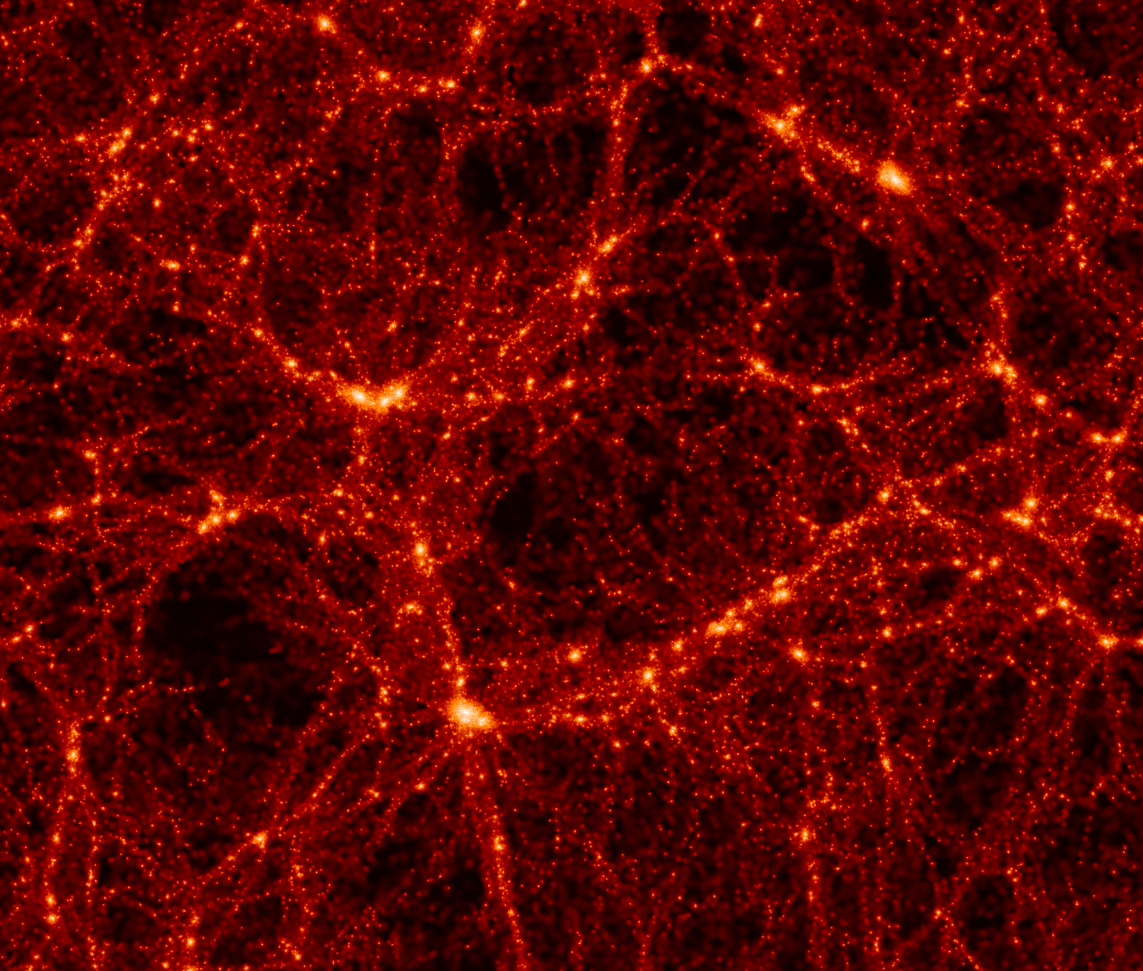
\includegraphics[scale = 0.3]{images/LCDM}
        \\ \caption{\textbf{Figure 1:} Complex structures that are a result of N-body simulations, \\the universe is observed to have a similar web-like structure}
        \label{fig:fig1}
    \end{center}
    
    
    \newpage
    
    \psection{Theory}

    \begin{itemize}
        \item We will contextualize the problem using the gravitational case. Treating the inputs as masses, positions and velocities of each body. \\

        \item The output would typically be the predictive trajectories as defined by solved functions of position and velocity. Assuming Newtonian physics. \\

        \item Suppose we have $n$ particles with masses $m_i$ and positions $\mathbf{r}_i(t)$. Then, particle $i$ has a gravitational force exerted on it by particle $j$. This is given by:

        \[ \mathbf{f}_{i,j}(t) = -\frac{Gm_i m_j}{|| \mathbf{r}_i(t) - \mathbf{r}_j(t) ||^3}(\mathbf{r}_i(t) - \mathbf{r}_j(t)) \]

        \item The total force on particle $i$ is then:

        \[ \mathbf{F}_i(t) = \sum_{j=0, j\ne i}^{n-1} \mathbf{f}_{i,j}(t) \]
        \noindent
        Which can be written as:
        \[ \mathbf{F}_i(t) = -Gm_i \sum_{j=0, j\ne i}^{n-1} \frac{ m_j}{|| \mathbf{r}_i(t) - \mathbf{r}_j(t) ||^3}(\mathbf{r}_i(t) - \mathbf{r}_j(t)) \]

        We know from Newton's law that $\mathbf{F} = m\mathbf{a}$, or in this context:
        \[ \mathbf{F}_i(t) = m_i\mathbf{\ddot{r}}_i(t) \]

        We can now substitute these relations to obtain a second order differential equation system:
        \[ \mathbf{\ddot{r}}_i(t) = -G \sum_{j=0, j\ne i}^{n-1} \frac{ m_j}{|| \mathbf{r}_i(t) - \mathbf{r}_j(t) ||^3}(\mathbf{r}_i(t) - \mathbf{r}_j(t)) \]
        \item This project, will hence focus on solving this exact problem.
        To make life easier, we will make some mathematical assumptions. Starting with the assumption that all the functions we will be dealing with, are functions of real numbers.
    \end{itemize}
    
    \newpage
    
    \psection{Numerics}
    
    \psubsection{Initial Approach}
    
    \begin{itemize}
        \item We know certain pieces of information, such as the conditions:
        \[ \mathbf{r}_i(0) = \mathbf{r}_0,\ \mathbf{\dot{r}}_i(0) = \mathbf{v}_0 \]
        \item Thus, we have an \emph{initial}-value problem.

        \item If the conditions are of the form:
        \[ \mathbf{r}_i(0) = \mathbf{r}_0,\ \mathbf{\dot{r}}_i(t) = \mathbf{r}_f \]
        \noindent
        we call it a \emph{boundary}-value problem.

        \item These problems are different enough that their numerical solutions are distinct.

        \item We will now explore methods of how we can solve these problems in different contexts.
        A naive approach to numerical integration for solving our obtained differential equations would follow the steps:
    \end{itemize}

    \noindent
    \indent \indent Given input data (Initial Conditions) \\
    \indent \indent \indent For each timestep $\Delta t$: \\
    \indent \indent \indent \indent For each particle $i$: \\
    \indent \indent \indent \indent \indent Compute $F_{\text{net}}(t)$ \\
    \indent \indent \indent \indent \indent Update $\mathbf{r_i}(t)$ and $\mathbf{\dot{r}}_i(t) = \mathbf{v}(t)$ for each particle $i$ \\
    \indent \indent \indent \indent \indent Return new positions and velocities

    \begin{itemize}
        \item This is called Euler's method! The way it was initially implemented was not ideal. It was a ``brute-force'' approach where the algorithm above was followed as is.
        \item This was a problem because when we tried to introduce a new algorithm (\textbf{RK4}), code had to be changed in a lot of places. \footnote{This was the route that we went and failed at miserably. The code was cryptic and very hard to understand.}
    \end{itemize}

    \psubsection{Euler's Method}
    \psubsubsection{Background}
    \begin{itemize}
        \item Euler's Method is designed to solve IVPs for first-order ordinary differential equations of the form:
        \[ \label{eq:3.1.1} y'=f(x,y),\quad y(x_0)=y_0 \]
        \item Where it can be used the approximate numerically the values of the solution of the ODE:
        \[ x_i=x_0+ih,\quad i=0,1, \dots,n, \nonumber \]
        \noindent
        Where:
        \[ h={\frac{b-x_0}{n}}.\nonumber \]

        \item We do this by starting with the tangent to an integral curve, given by:
        \[ \label{eq:3.1.2} y=y(x_i)+f(x_i,y(x_i))(x-x_i) \]

        \item Setting the step $(x-x_i)$ to $h$, and using the IC $y(x_0) = y_0$ we can give a general expression for all solutions to $y(x)$ as:
        \[ \label{eq:3.1.4} y_{i+1}=y_i+hf(x_i,y_i),\quad 0\le i\le n-1. \]

        \item However, the problem we intend to solve, always involves second-order ODEs, as shown before. Luckily, there is a way to convert any such DE into two coupled first-order ODEs. Consider a generalized form of the n-body ODE we defined earlier:
        \[  \mathbf{\ddot{r}}(t) = -\mathbf{r}(t) \]

        \item We can convert this to a system of $2n$ first order ODEs:
        \[ \mathbf{\dot{r}_i}(t) = \mathbf{v}_i(t) \]
        \[ \mathbf{\dot{v}_i}(t) = \frac{1}{m_i}\mathbf{F}_i(t) \]

        Under the initial conditions:
        \[ \mathbf{r}_i(0) = \mathbf{r}_i,0, \ \mathbf{v}_i(0) = \mathbf{v}_i,0 \]

        Allowing us to numerically solve any system.
    \end{itemize}
    
    \psubsubsection{\texttt{Python}}

    \begin{itemize}
        \item After failing at morphing the previous adaptation to swap out algorithms, it was clear that there was a need for a revamp.
        \item First, we seperated out the algorithm, instead it being embedded in the \texttt{System} class, we pulled it out into a (here) \texttt{EulerUtils} class, this was then passed to \texttt{System}.
        \item The main takeaway was: \textbf{Each Algorithm can spit out an updated vector; it needs to know how to ``differentiate'' the initial vector and the initial vector itself.}
        \item Here, the algorithm itself doesn't care what ``differentiate'' means, it's an implementation detail for all it cares. What it means for us is that we show it a way of getting (for example) $dv$ given $v$ (conveniently, $dv$ can be inferred from the acceleration, $\frac{dv}{dt}$).
        \item The algorithm looks like:
    \end{itemize}
    \begin{lstlisting}[language=Python, caption=Euler's method]
def Euler_algorithm(f, t_i, y_i, dt):
    y_i_plus_1 = y_i + dt*f(t_i, y_i)
    return y_i_plus_1
    \end{lstlisting}
    \begin{itemize}
        \item Here, \texttt{y\_i} is the vector which we want to calculate the next step of; \texttt{t\_i} is the initial time; \texttt{f} calculates the derivative (for a given \texttt{t} and \texttt{y}); and \texttt{dt} is the time differential.
        \item Now let's look at what \texttt{System} looks like:
    \end{itemize}

    \begin{lstlisting}[language=Python, caption=System]
class System:
    def __init__(self,
                 dt,
                 algorithm,
                 bodies=[],
                 law=None):
        self.dt = dt
        self.algorithm = algorithm
        self.bodies = np.array(bodies)
        self.law = law

    # Convinience method to get the latest vector for the algorithm(s) to use.
    def latest_vector(self):
        vec = np.array([self.bodies[0].position[-1], self.bodies[0].velocity[-1]])
        for body in self.bodies[1:]:
            vec = np.append(vec, [body.position[-1], body.velocity[-1]], axis=0)
        return vec

    def initial_vector(self):
        vec = np.array([self.bodies[0].position[0], self.bodies[0].velocity[0]])
        for body in self.bodies[1:]:
            vec = np.append(vec, [body.position[0], body.velocity[0]], axis=0)
        return vec

    # Builds a list of masses of the bodies that make up the system.
    def masses(self):
        return np.array(list(map(lambda body: body.mass, self.bodies)))

    def derivator(self, t, y):
        G = coconst.G.value
        # Here, we need to tell RK4 how to differentiate y, and then return it.
        y_prime = np.zeros_like(y)
        # Even indices of `y_prime` are just equal to the next index in y.
        for i, _y in enumerate(y):
            if i % 2 == 0:
                y_prime[i] = y[i + 1]

        for j, _y2 in enumerate(y):
            if j % 2 != 0:
                for other_body in np.delete(self.bodies, int((j - 1)/2)):
                    y_prime[j] += -G*other_body.mass*(y[j - 1] - other_body.position[-1])/(np.linalg.norm(y[j - 1] - other_body.position[-1]))**3


        # Now that we filled in all the blanks, we can return `y_prime`.
        return y_prime

    def simulate(self, until=0.0):
        t = 0.0
        while t < until:
            # This is the next step of our special vector.
            step = self.algorithm(f=self.derivator,
                                      t_i=0.,
                                      y_i=self.latest_vector(),
                                      dt=self.dt)

            for i, body in enumerate(self.bodies):
                body.position = np.append(body.position, [step[i*2]], axis=0)
                body.velocity = np.append(body.velocity, [step[i*2 + 1]], axis=0)
            t += self.dt
    \end{lstlisting}
    \begin{itemize}
        \item Okay, that's a lot to unpack. Most of the methods are self explanatory, the only methods that really concern us are \texttt{derivator} and \texttt{simulate}:
        \begin{itemize}
            \item \texttt{derivator}: Recall how we needed to tell the algorithm how to calculate the derivative of a given \texttt{y} vector. This essentially maps $y$ to $y'$:
            \[ \begin{pmatrix} x_i \\ \dot{x}_i \end{pmatrix} \rightarrow \begin{pmatrix} \dot{x}_i \\ \ddot{x}_i \end{pmatrix} \]
            Notice that one of the vector entries is simply copied over to a different index ($\dot{x}_i$). This is exactly what's happening in line 36 of Listing 2. For the second entry, $\ddot{x}_i$, we make use of the law of the system and calculate it explicitly:
            \[ a_i = \ddot{x}_i = \sum_{j}^{} \frac{-G m_j (\vec{x_i} - \vec{x_j})}{||\vec{x_i} - \vec{x_j}||^3}  \]
            \textbf{We (the algorithm rather) now have the differentiated vector!}
            \item \texttt{simulate}: This is where we call the algorithm and pass the parameters it needs: The ``derivator'' that we implemented earlier and the initial conditions which can be found with the convenience methods \texttt{latest\_vector} and \texttt{initial\_vector}.
        \end{itemize}
        \item That's all!
    \end{itemize}
    
    \psubsection{RK4 Integration}

    \psubsubsection{Background}
    \begin{itemize}
        \item Consider the same IVP as before:
        \[ \label{eq:3.1.1} y'=f(x,y),\quad y(x_0)=y_0 \]
        We pick a step-size $h>0$ and define:
        \[ y_{n+1} = y_n + \frac{1}{6}(k_1 + 2k_2 + 2k_3 + k_4)h, \]
        \[ t_{n+1} = t_n + h, \ n= 0,1,2,3,\dots,n \]

        Where:
        \[ k_{1}=h f\left(t_{n}, y_{n}\right) \]
        \[ k_{2}=h f\left(t_{n}+\frac{h}{2}, y_{n}+\frac{1}{2} k_{1}\right) \]
        \[ k_{3}=h f\left(t_{n}+\frac{h}{2}, y_{n}+\frac{1}{2} k_{2}\right) \]
        \[ k_{4}=h f\left(t_{n}+h, y_{n}+k_{3}\right) \]

        \item However, as we reduce a second order ODE to 2 couples first order ODEs:
        \[  \mathbf{\dot{r}_i}(t) = \mathbf{v}_i(t) \]
        \[ \mathbf{\dot{v}_i}(t) = \frac{1}{m_i}\mathbf{F}_i(t) \]

        The k parameters of the RK4 solutions change to two sets, one for approximations of position, and one for velocity. Given as follows:
        \[ k_{1}=h \mathbf{v}\left(t_{i}, x_{i}, v_{i}\right) \]
        \[ k_{2}=h \mathbf{v}\left(t_{i} + \frac{h}{2}, x_{i} +\frac{hk_1}{2}, v_{i}+\frac{hl_1}{2}\right) \]
        \[ k_{3}=h \mathbf{v}\left(t_{i} + \frac{h}{2}, x_{i} +\frac{hk_2}{2}, v_{i}+\frac{hl_2}{2}\right) \]
        \[ k_{4}=h \mathbf{v}\left(t_{i}+h, x_{i}+hk_3, v_{i}+hl_3\right) \]
        \[ x_{i+1} = x_i + \frac{h}{6} \left( k_1 + 2k_2 + 2k_3 + k_4 \right) \]

        And:
        \[ l_{1}=\frac{h}{m_i} \mathbf{F}\left(t_{i}, x_{i}, v_{i}\right) \]
        \[ k_{2}=\frac{h}{m_i} \mathbf{F}\left(t_{i} + \frac{h}{2}, x_{i} +\frac{hk_1}{2}, v_{i}+\frac{hl_1}{2}\right) \]
        \[ k_{3}=\frac{h}{m_i} \mathbf{F}\left(t_{i} + \frac{h}{2}, x_{i} +\frac{hk_2}{2}, v_{i}+\frac{hl_2}{2}\right) \]
        \[ k_{4}=\frac{h}{m_i} \mathbf{F}\left(t_{i}+h, x_{i}+hk_3, v_{i}+hl_3\right) \]
        \[ v_{i+1} = v_i + \frac{h}{6} \left( l_1 + 2l_2 + 2l_3 + l_4 \right) \]
    \end{itemize}
    
    \psubsubsection{\texttt{Python}}
    \begin{itemize}
        \item The algorithm above was implemented in its own file (as was done for Euler's method in the previous section):
    \end{itemize}
    \begin{lstlisting}[language=Python, caption=RK4 integration]
def RK4_algorithm(f, t_i, y_i, dt):
    '''
    For steps involved, refer to: https://en.wikipedia.org/wiki/Runge%E2%80%93Kutta_methods.
    '''
    # Know k_1y:
    k_1y = f(t_i, y_i)

    # Find k_2y:
    k_2y = f(t_i + dt/2, y_i + dt*k_1y/2)

    # Find k_3y:
    k_3y = f(t_i + dt/2, y_i + dt*k_2y/2)

    # Find k_4y:
    k_4y = f(t_i + dt, y_i + dt*k_3y)

    # Find y_{i + 1}:
    y_i_plus_1 = y_i + (dt/6)*(k_1y + 2*k_2y + 2*k_3y + k_4y)
    return y_i_plus_1
    \end{lstlisting}
    \begin{itemize}
        \item Something extremely important to notice here is that \textbf{this has the exact same inputs and outputs of \texttt{Euler\_algorithm} in Listing 1!}
        \item Because of the way we abstracted the implementation detail of the algorithm from \texttt{System} in this approach, this meant that all we had to do was pass this algorithm to the constructor of \texttt{System}.
    \end{itemize}

    \newpage

    \psection{Tests}

    \noindent
    Now, let's actually use the classes and algorithm that we built to simulate specific systems.
    \psubsection{Earth-Sun}

    \psubsubsection{Classical 2-Body Problem}
    \begin{itemize}
        \item We will use the famous Kepler's problem as the first test to gauge how well our numerical methods work.
        \item In classical mechanics, the Kepler problem is essentially a special case of the 2-body problem in which bodies interact a radial inverse square potential. The problem is to find their position/speeds as a time series, given their masses, and initial positions, velocities.
        \item The central force between two objects is defined as:
        \[ \mathbf{F} = \frac{k}{r^2} (\mathbf{\hat{r}}) \]
        Which corresponds to the scalar potential:
        \[ V(r) = \frac{k}{r} \]
        The equation of motion of a point mass in a particle is given by:
        \[ m\frac{d^2 r}{dt^2} - mr \omega^2 = m\frac{d^2 r}{dt^2} - \frac{L^2}{mr^3} = -\frac{dV}{dr} \]
        Where $w = \frac{d\theta}{dt}$ and $L= mr^2 \omega$ (angular momentum) is conserved.\\
        \item This DE is of the same form as our general n-body ODE. Under the condition that $L$ be non-zero (which it is), we can convert this DE in polar coordinates, with $r$ being a $r(\theta)$ instead of $r(t)$:
        \[ \frac{d}{dt} = \frac{L}{mr^{2}} \frac{d}{d\theta} \]
        \item Making the DE independent of time:
        \[ \frac{L}{r^2} \frac{d}{d\theta} \left( \frac{L}{mr^2} \frac{dr}{d\theta} \right)- \frac{L^2}{mr^3} = -\frac{dV}{dr} \]
        \item Finally we use change of variable $u = \frac{1}{r}$ to make the ODE quasi-linear:
        \[ \frac{d^2 u}{d\theta^2} + u = -\frac{m}{L^2}  \frac{d}{du} V\left( \frac 1 u\right) = -\frac{km}{L^2} \]
        \item Which can be analytically solved to give us:
        \[ u \equiv \frac{1}{r} = -\frac{km}{L^2} \left[ 1 + e \cos(\theta - \theta_0) \right] \]
        \item Here, $e$ represents the eccentricity of the orbit, with it ranging between $0$ and $1$. The lower bound corresponding to perfect circular motion, and the upper bound corresponding to an unbound parabola. It relates to energy as:
        \[ e = \sqrt{1 + \frac{2EL^2}{k^2 m}} \]

    Note that the eccentricity and angular momentum of the Earth are known to be:
        \[ e = 0.0167 \]
        \[ L =  2.7\times10^{40} \text{kg} \frac{\text{m}^2}{\text{s}} \]

    We can use this solution to model the Earth-Sun system.
    \end{itemize}

    \psubsubsection{Euler's Method}

    \begin{itemize}
        \item The first system that is the easiest to test is the Earth-Sun system, since we know exactly what to expect in this case: The Earth revolves around the Sun at 1AU.
        \item We first create the objects \texttt{earth} and \texttt{sun} using a \texttt{Body} class, all this does is arrange the meta-data associated with a body in a neat way, using:
    \end{itemize}
    \begin{lstlisting}[language=Python, caption=\texttt{Body} class]
class Body:
    def __init__(self,
                 name,
                 mass=0.0,
                 position=[[0, 0]],
                 velocity=[[0, 0]],
                 net_force=[0.0, 0.0]):
        self.name = name
        self.mass = mass
        self.position = np.array(position)
        self.velocity = np.array(velocity)
        self.net_force = np.array(net_force)
    \end{lstlisting}
    \begin{itemize}
        \item We can hence create instances of this class as:
    \end{itemize}
    \begin{lstlisting}[language=Python, caption=\texttt{Body} objects]
earth = Body(name="Earth",
             mass=aconst.M_earth.value,
             position=[[aconst.au.value, 0]],
             velocity=[[0, 29784.8]])

halley = Body(name="Halley",
             mass=2.2e14,
             position=[[0.5871*aconst.au.value, 0]],
             velocity=[[0, 53545]])


sun = Body(name="Sun",
           mass=aconst.M_sun.value)

jwst = Body(name="JWST",
                 mass=6500,
                 position=[L1],
                 velocity=[[0, 0]])
    \end{lstlisting}
    \begin{itemize}
        \item We create an instance of \texttt{System} and pass a list of the \texttt{Body} instances that we want in the system. Let's first try an Earth-Sun system: \footnote{Here, the \texttt{law} parameter is not used, this is beyond the scope of this project where we want might consider a system governed by a law that might not be Newtonian. It is however, still a good idea to generalize this.}
    \end{itemize}

    \begin{lstlisting}[language=Python, caption=Earth-Sun system]
bodies = [earth, sun]
system = System(bodies=bodies,
                dt=100000,
                algorithm=eu.Euler_algorithm,
                # Not used
                law=lambda m1, m2, x1, x2: ((coconst.G.value*m1*m2)/((lin.norm(x2 - x1))**3)) * (x2 - x1))
    \end{lstlisting}

    \begin{itemize}
        \item Now, we can use the \texttt{simulate} method discussed earlier to mutate the positions and velocities of \texttt{bodies} (for 1 year):
    \end{itemize}
    \begin{lstlisting}[language=Python, caption=Simulate the system for a year]
system.simulate(until=3.154e7)
    \end{lstlisting}
    \begin{itemize}
        \item There is also a \texttt{PlotUtils} class which handles plotting for this project. Upon plotting the trajectories of \texttt{earth} and \texttt{sun} using Euler integration, we get:
    \end{itemize}

    \begin{center}
        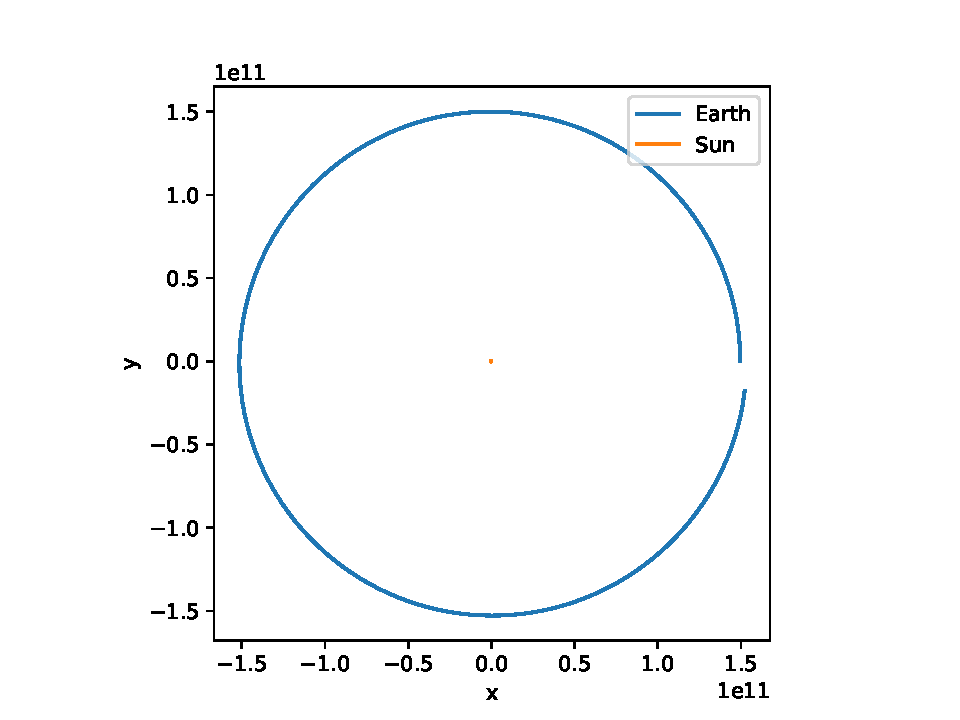
\includegraphics[scale = 1]{images/euler_earth_sun}
        \\ \caption{\textbf{Figure 2:} Earth-Sun simulation with Euler's method (1 year)}
        \label{fig:fig2}
    \end{center}

    \begin{itemize}
        \item Notice that the Earth doesn't quite make it to the initial spot and the radius of its orbit increases.
        \item This suggests that it ``loses'' energy. The loss can be attributed to the fact that Euler's method linearly interpolates the differential trajectories. Since the radius has been increasing over the ``circle'', it doesn't make it to the initial position and drifts away.
        \item This is more apparent if we run the simulation for say, 20 years (with the same time step):
    \end{itemize}

    \begin{center}
        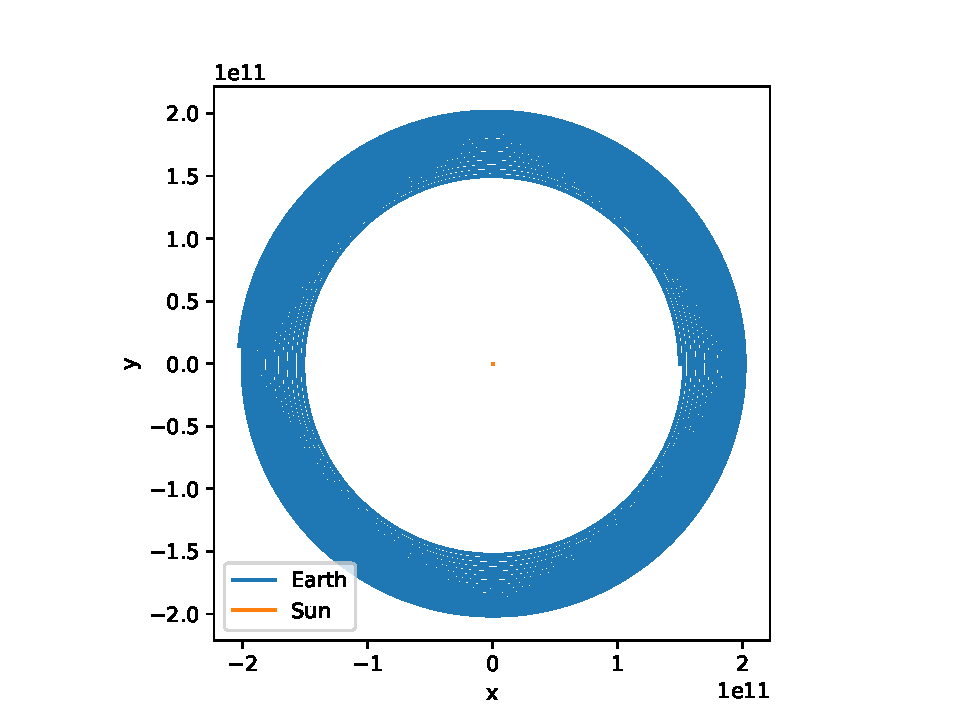
\includegraphics[scale = 1]{images/euler_earth_sun_20_years}
        \\ \caption{\textbf{Figure 3:} Earth-Sun simulation with Euler's method (20 years)}
        \label{fig:fig3}
    \end{center}

    \begin{itemize}
        \item This drift is a result of the integration method used. The way we fix it is to introduce a better algorithm, \textbf{RK4}!
    \end{itemize}
    
    \psubsubsection{RK4 Integration}

    \begin{itemize}
        \item Let's run the previous simulation (1 year, using the same time step, $dt = 10000$s) using RK4\footnote{Recall that all we need to do is swap the algorithm that we pass to \texttt{Sysstem}.}. We get the following plot:
    \end{itemize}

    \begin{center}
        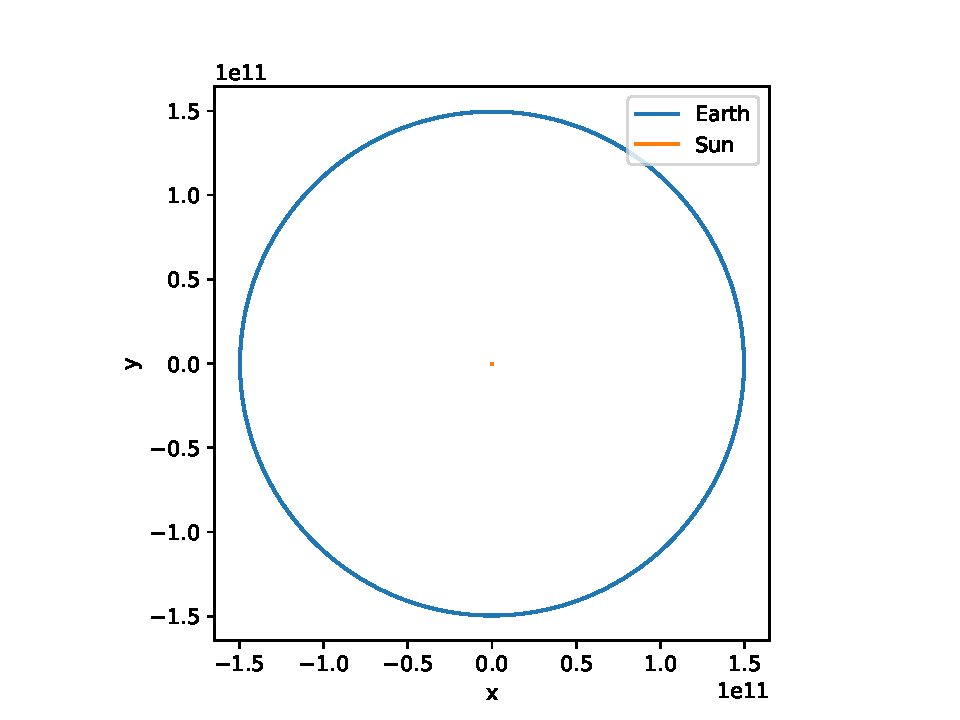
\includegraphics[scale = 0.8]{images/rk4_earth_sun}
        \\ \caption{\textbf{Figure 4:} Earth-Sun simulation with RK4 integration (1 year)}
        \label{fig:fig4}
    \end{center}

    \begin{itemize}
        \item Because of how the RK4 method averages over smaller steps in $dt$, we see immediately from Figure 4 that this is a much better result, earth seems to return to nearly the same initial position after 1 year (as we would expect).
        \item Now, let's run this for 50 years to re-affirm our analysis.
    \end{itemize}

    \begin{center}
        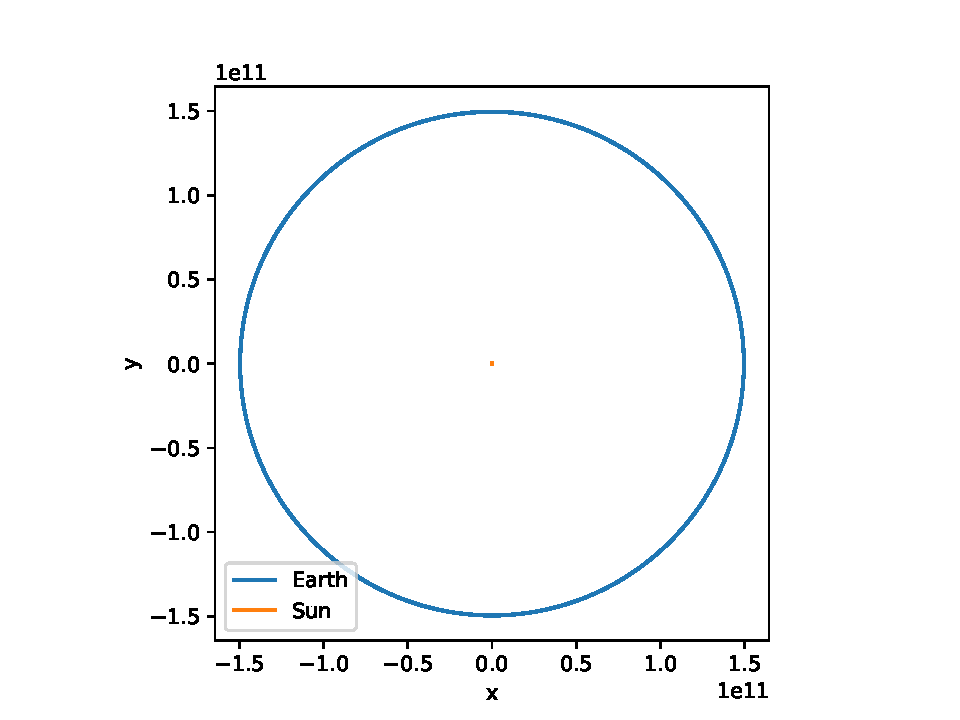
\includegraphics[scale = 0.8]{images/rk4_earth_sun_50_years}
        \\ \caption{\textbf{Figure 5:} Earth-Sun simulation with RK4 integration (\textbf{50 years}!)}
        \label{fig:fig5}
    \end{center}

    \begin{itemize}
        \item And we don't drift away, even after 50 years (the orbits overlap)!\footnote{This ran for longer than Euler's method, since the time complexity is $\approx$O($n^2$). But humanity survives!}
    \end{itemize}
    
    \psubsection{Halley-Earth-Sun}
    \begin{itemize}
        \item As another sanity check, we can use RK4 on the Earth-Sun system along with Halley's comet. the period of Halley's comet is known to be approximately 76 years. We hence add the \texttt{Body} instance of this comet, \texttt{halley}, to the list of bodies and pass it to the \texttt{system}:
    \end{itemize}

    \begin{lstlisting}[language=Python, caption=Simulate the system for a year]
    earth = Body(name="Earth",
                 mass=aconst.M_earth.value,
                 position=[[aconst.au.value, 0]],
                 velocity=[[0, 29784.8]])

    halley = Body(name="Halley",
                  mass=2.2e14,
                  position=[[0.5871*aconst.au.value, 0]],
                  velocity=[[0, 53545]])

    sun = Body(name="Sun",
               mass=aconst.M_sun.value)

    bodies = [halley, earth, sun]

    system = System(bodies=bodies,
                    dt=100000,
                    algorithm=rk.RK4_algorithm,
                    law=lambda m1, m2, x1, x2: ((coconst.G.value*m1*m2)/((lin.norm(x2 - x1))**3)) * (x2 - x1))

    # 76 Years
    system.simulate(until=3.154e7*76)
    \end{lstlisting}

    \begin{itemize}
        \item Notice that we increased the time step so we can generate the plot in a reasonable amount of time. Upon plotting the trajectories of the bodies using RK4, we get:
    \end{itemize}

    \begin{center}
        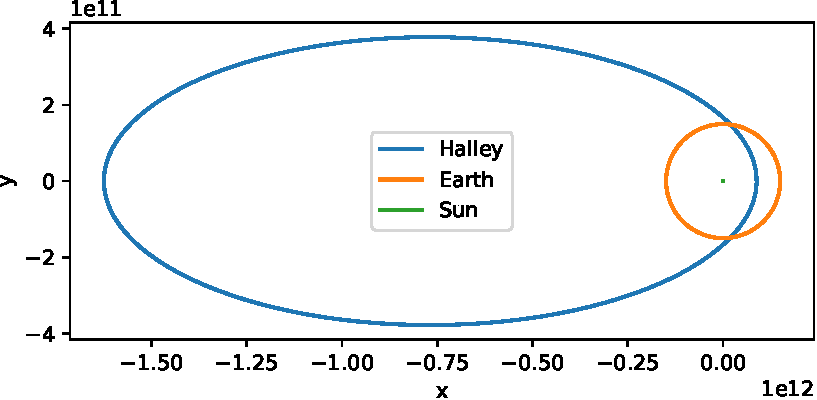
\includegraphics[scale = 1.1]{images/halley-crop}
        \\ \caption{\textbf{Figure 6:} Halley-Earth-Sun simulation with RK4 integration (\textbf{75 years}!)}
        \label{fig:fig6}
    \end{center}

    \begin{itemize}
        \item Halley's comet returns to near-Earth so humanity can observe it once in a lifetime!\footnote{The Aphelion and Perhelion of the comet also appear to be accurate.}
    \end{itemize}

    \newpage

    \psection{Studies}
    
    \psubsection{Lagrange Points}

    \psubsubsection{Background}
    \begin{itemize}
        \item As discussed earlier, the N-body problem has no analytical solutions in any cases involving 3 or more bodies. However, we do have some information from higher order problems that we can use to test our methods of integration.
        \item One such example are the Lagrange points and how they appear in the restricted 3 body problem. This problem refers to a special case of the 3-body problem where 2 of the masses involved are much bigger than the third. Turns out that the geometry of this problem reveals the existence of 5 equilibrium points in space in the vicinity of the 2 massive bodies. These are called Lagrange points, and their coordinates can be found analytically.
        \item Consider hence, the restricted 3 body problem. With 3 masses $M_1$, $M_2$ and $m$, where $M_1, M_2 \gg m$, and their respective positions are given by $r_1$, $r_2$, $r$. The total force exerted on the small mass $m$ is hence:
        \[ \mathbf{F}(t) = m\frac{d^2 \mathbf{r}(t)}{dt^2} = -\frac{G M_1 m}{|| \mathbf{r}(t) - \mathbf{r_1}(t) ||^3}(\mathbf{r}(t) - \mathbf{r_1}_j(t))-\frac{G M_2 m}{|| \mathbf{r}(t) - \mathbf{r_2}(t) ||^3}(\mathbf{r}(t) - \mathbf{r_2}_j(t)) \]
        \item Once again, we have a variation of our n-body ODE. However, only stationary solutions are possible for this version. The process involves conversion to a rotating reference frame. We will not be listing the complete derivation, however the final relation is of the form:
        \[ \mathbf{F}_{\Omega} = \Omega^2 \left(x-\frac{\beta R^3(x+\alpha R)}{((x+\alpha R)^2+y^2)^{3/2}}
        -\frac{\alpha R^3(x-\beta R)}{((x-\beta R)^2+y^2)^{3/2}}\right) \hat{\mathbf{i}} +\]
        \[\Omega^2 \left(x-\frac{\beta R^3 y}{((x+\alpha R)^2+y^2)^{3/2}}
        -\frac{\alpha R^3 y}{((x-\beta R)^2+y^2)^{3/2}}\right) \hat{\mathbf{j}} \]

        where:
        \[ \alpha = \frac{M_2}{M_1+M_2}, \ \ \beta = \frac{M_1}{M_1+M_2} \]

        \item In the limit $\alpha \ll 1$, we get the following Lagrange points:
        \[ L1: \bigg( R \bigg( 1-\bigg(\frac{\alpha}{3}\bigg)^{\frac{1}{3}} \bigg), 0 \bigg) \]
        \[ L2: \bigg( R \bigg( 1+\bigg(\frac{\alpha}{3}\bigg)^{\frac{1}{3}} \bigg), 0 \bigg) \]
        \[ L3: \bigg( -R \bigg( 1+\frac{15 \alpha}{12} \bigg), 0 \bigg) \]
        \[ L4: \bigg( \frac{R}{2} \bigg(\frac{M_1-M_2}{M_1+M_2} \bigg), \frac{R\sqrt{3}}{2} \bigg) \]
        \[ L5: \bigg( \frac{R}{2} \bigg(\frac{M_1-M_2}{M_1+M_2} \bigg), -\frac{R\sqrt{3}}{2} \bigg) \]

        \item For the Earth-Sun system:
        \[ \alpha \approx 3\times10^{-6} \]
        \[ R = 1 \text{AU} = 1.5 \times 10^8 \text{km} \]
    \end{itemize}

    \psubsubsection{\texttt{Python}}
    \begin{itemize}
        \item The James Webb Space Telescope was positioned in a halo orbit about L2 on January 24, 2022. We can create a \texttt{jwst} object and set it in motion at $\approx$100$\frac{\text{m}}{\text{s}}$ to see how it behaves at L2:
    \end{itemize}
    \begin{lstlisting}[language=Python, caption=Simulate the system for 10 years]
# Lagrange points
alpha = 3e-6
R = aconst.au.value
L2 = [R * (1 + (alpha/3)**(1/3)), 0]

jwst = Body(name="JWST",
                 mass=0,
                 position=[[L2[0] - (832e6 - 250e6)/2, 0]],
                 velocity=[[0, 29784.8 + 93]])

bodies = [jwst, earth, sun]

system = System(bodies=bodies,
                dt=10000,
                algorithm=rk.RK4_algorithm,
                law=lambda m1, m2, x1, x2: ((coconst.G.value*m1*m2)/((lin.norm(x2 - x1))**3)) * (x2 - x1))

# 10 Years
system.simulate(until=3.154e7*10)
    \end{lstlisting}

    \begin{itemize}
        \item On plotting the trajectory of \texttt{jwst} around the sun for these 10 years, we get:
    \end{itemize}

    \begin{center}
        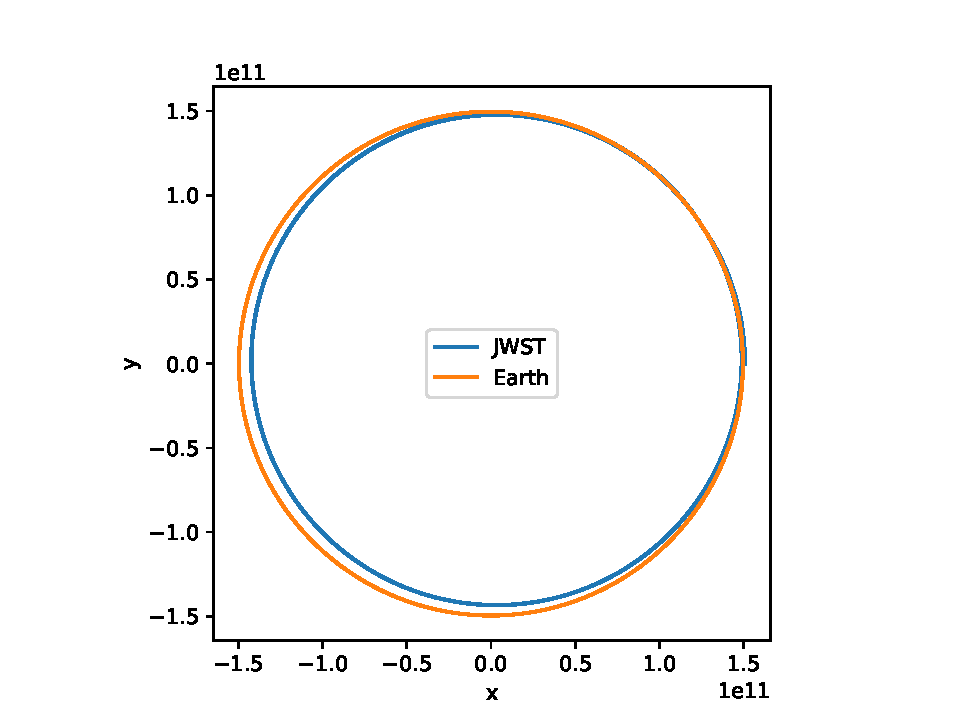
\includegraphics[scale = 0.8]{images/rk4_jwst}
        \\ \caption{\textbf{Figure 7:} JWST-Earth-Sun simulation with RK4 integration (\textbf{10 years})}
        \label{fig:fig7}
    \end{center}
    
    \newpage
    
    \psection{Conclusion}
    \psubsection{Algorithms}
    \begin{itemize}
        \item In this report, we initially ``brute-forced'' Euler's method to solve a coupled DE (first version).
        \item After realizing that it doesn't scale well, (for instance, if the algorithm needed to be swapped out for another) we refactored the code to enable the algorithm to be passed as a constructor parameter to the \texttt{System} instance.
        \item This change came about after the stark realization that the system didn't (and shouldn't) care about the algorithm at hand. It is only concerned with the gravitational law.
        \item Similarly, the algorithm needs to know how to differentiate the state of the system to produce the next step in the state.
        \item After generalizing the system to allow for these, we could easily swap out Euler for RK4 (or any other algorithm for that matter). Both \textbf{Euler's method} and \textbf{RK4 integration} were implemented in their own \texttt{Util} files.
        \item RK4 was considerably slower than Euler but was more accurate since it interpolated using more granular time steps (averaged over them). This ``prevented'' energy loss over the time scales used and hence fit our needs better.
    \end{itemize}
    \psubsection{Tests}
    \begin{itemize}
        \item Both algorithms were tested on Earth-Sun and Halley-Earth-Sun systems. We saw that the earth continued to rotate in the same orbit for a 50 year simulation when RK4 integration was used.
        \item Further, Halley's comet returned to it's initial position (0.5871 AU, from the Sun and between the Earth and the Sun) over it's orbit period of $\approx$76 years. All the while, Earth rotated in its orbit (when RK4 was used). In contrast to this, Euler produced the following inaccurate result:
    \end{itemize}
    \begin{center}
        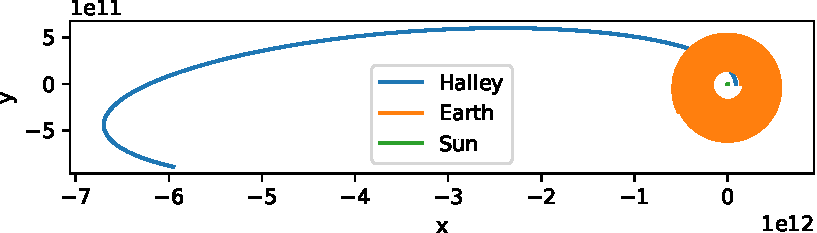
\includegraphics[scale = 1.2]{images/inaccurate-crop}
        \\ \caption{\textbf{Figure 8:} Halley-Earth-Sun simulation with Euler's method}
        \label{fig:fig8}
    \end{center}

    \psubsection{Studies}
    \begin{itemize}
        \item Finally, we took a brief look at how the JWST satellite behaved around the L2 Lagrange point which it orbits.
        \item The plot revealed that it stays in orbit around L2 over the 10-year simulation using RK4.
        \item Changing its momentum causes it to stray away from the L2 point and drift away from the Earth-Sun system:
    \end{itemize}
    \begin{center}
        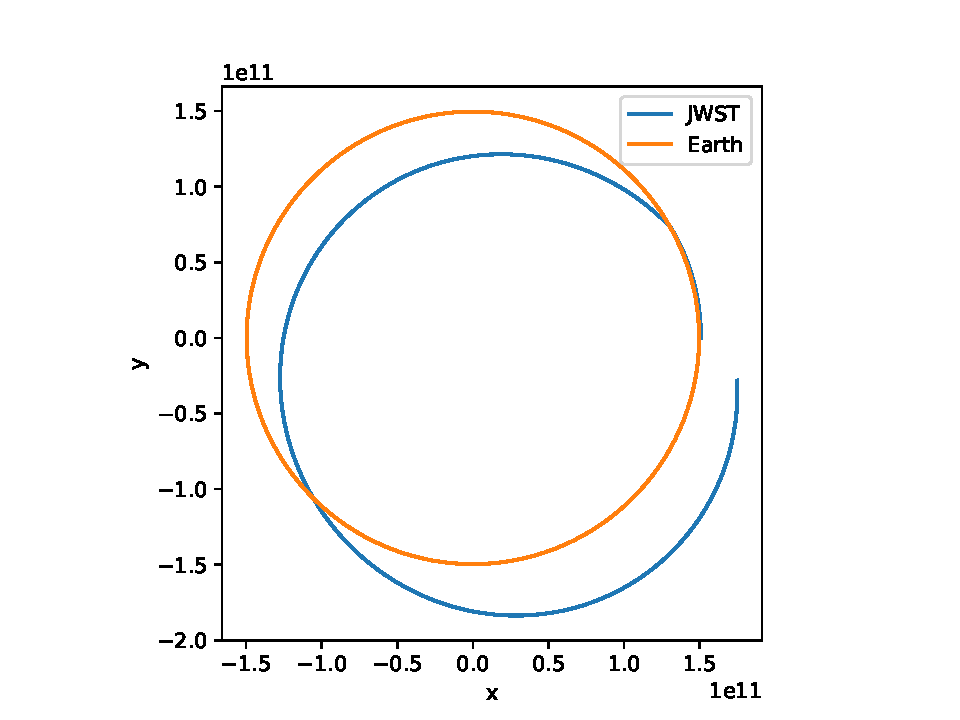
\includegraphics[scale = 1]{images/jwst_broken}
        \\ \caption{\textbf{Figure 9:} JWST drifting away}
        \label{fig:fig9}
    \end{center}
\end{document}
